\chapter{Описание метода решения}
\label{chap:def}
    \section{Математический аппарат} \\
    \paragraph{Метрики}
    \noindent \\
        
    \noindent
        В работе используются следующие метрики: \\
        \begin{enumerate}
            \item MultiClass:
             $$
            \sum_{i=1}^{N} w_{i} \log \left(\frac{e^{a_{i t_{i}}}}{\sum_{j=0}^{M-1} e^{a_{i j}}}\right)
            $$
            $$
            \sum_{i=1}^{N} w_{i}$$
            $$
            t \in\{0, \ldots, M-1\}
            $$
            \item MultiClassOneVsAll: 
            $$
            \frac{\frac{1}{M} \sum_{i=1}^{N} w_{i} \sum_{j=0}^{M-1}\left[j=t_{i}\right] \log \left(p_{i j}\right)+\left[j \neq t_{i}\right] \log \left(1-p_{i j}\right)}{\sum_{i=1}^{N} w_{i}}
            $$
            $$          
            t \in\{0, \ldots, M-1\}
            $$
            \item Total F1 weighted:
            $$ 
            \frac{\sum_{i=1}^{M} w_{i} F 1_{i}}{\sum_{i=1}^{M} w_{i}}
            $$
            \item MCC: 
            $$
            \frac{\sum_{k} \sum_{l} \sum_{m} C_{k k} C_{l m}-C_{k l} C_{m k}}{\sqrt{\sum_{k}\left(\sum_{l} C_{k l}\right)\left(\sum_{k^{\prime} \mid k^{\prime} \neq k} \sum_{l^{\prime}} C_{k^{\prime} l^{\prime}}\right)} \sqrt{\sum_{k}\left(\sum_{l} C_{l k}\right)\left(\sum_{k^{\prime} \mid k^{\prime} \neq k} \sum_{l^{\prime}} C_{l^{\prime} k^{\prime}}\right)}}
            $$
            \item Accuracy:
            $$
            \frac{\sum_{i=1}^{N} w_{i}\left[\operatorname{argmax}_{j=0, \ldots, M-1}\left(a_{i j}\right)==t_{i}\right]}{\sum_{i=1}^{N} w_{i}}
            $$
            $$
            t \in\{0, \ldots, M-1\}
            $$
            \item Hinge loss:
            $$
            \ell(y)=\max (0,1-t \cdot y)
            $$
            \item Hamming loss:
            $$
            \sum_{i=1}^{N} w_{i}\left[\operatorname{argmax}_{j=0, \ldots, M-1}\left(a_{i j}\right) \neq t_{i}\right]
            $$
            $$
            \sum_{i=1}^{N} w_{i}
            $$
            \item Zero One loss:
            $$1 - Accuracy$$
            \item Kappa:
            $$
            1-\frac{1-Accuracy }{1-RAccuracy }
            $$
$$RAccuracy =\frac{\sum_{k=0}^{M-1} n_{k_{a}} n_{k_{t}}}{\left(\sum_{i=1}^{N} w_{i}\right)^{2}}
$$
            \item WKappa:
            $$
\kappa_{w}=\frac{p_{o}-p_{e}}{1-p_{e}}
$$
где $p_{0}=\sum_{i=1}^{K} \sum_{j=1}^{K} w_{i j} p_{i j}$ и $p_{e}=\sum_{i=1}^{K} \sum_{j=1}^{K} w_{i j} p_{i . p} p_{. j}$ при $0 \leq w_{i j} \leq 1$ и $w_{j j}=1(i, j=1, \cdots, K)$, или
$$
\kappa_{w}=1-\frac{q_{o}}{q_{e}}
$$
где $q_{0}=\sum_{i=1}^{K} \sum_{j=1}^{K} v_{i j} p_{i j}$ и  $q_{e}=\sum_{i=1}^{K} \sum_{j=1}^{K} v_{i j} p_{i .} p_{. j}$ при $0 \leq v_{i j} \leq 1$ и $v_{j j}=0(i, j=1, \cdots, K)$. 
            \item AUC$\mu$:
            $$\mathrm{AUC}=\frac{1}{n_{+} n_{-}} \sum_{\hat{p}^{(i)} \in D^{+}} \sum_{\hat{p}^{(j)} \in D^{-}} \tilde{I}\left(\hat{p}^{(i)}-\hat{p}^{(j)}\right)$$
            $$S(i, j)=\frac{1}{n_{i} n_{j}} \sum_{a \in D^{i}, b \in D^{j}} \tilde{I} \circ O\left(\mathbf{y}^{(a)}, \mathbf{y}^{(b)}, \hat{\mathbf{p}}^{(a)}, \hat{\mathbf{p}}^{(b)}, \mathbf{v}_{i, j}\right)$$
            $$\mathrm{AUC}_{\mu}=\frac{2}{K(K-1)} \sum_{i<j} S(i, j)$$
        \end{enumerate}
        
        \newpage
        \paragraph
        {
        Метрический классификатор
        }
        \noindent\\
        
        \noindent
        Для произвольного объекта $a \in X$ расположим элементы обучающей выборки $x_{1}, \ldots, x_{\ell}$ в порядке возрастания расстояний до $a$ :
$$
\rho\left(a, x_{a}^{(1)}\right) \leqslant \rho\left(a, x_{a}^{(2)}\right) \leqslant \cdots \leqslant \rho\left(a, x_{a}^{(\ell)}\right)
$$
где через $x_{a}^{(i)}$ обозначается $i$-й сосед объекта $a$. Соответственно, ответ на $i$-м соседе объекта $a$ есть $y_{a}^{(i)}=y^{*}\left(x_{a}^{(i)}\right)$. Таким образом, любой объект $a \in X$ порождает свою перенумерацию выборки.

\emph{Определение.} Метрический алгоритм классификации с обучающей выборкой $X^{\ell}$ относит объект $x$ к тому классу $y \in Y$, для которого суммарный вес ближайших обучающих объектов $\Gamma_{y}\left(x, X^{\ell}\right)$ максимален:
$$
a\left(x ; X^{\ell}\right)=\arg \max _{y \in Y} \Gamma_{y}\left(x, X^{\ell}\right) ; \quad \Gamma_{y}\left(x, X^{\ell}\right)=\sum_{i=1}^{\ell}\left[y_{x}^{(i)}=y\right] w(i, x),
$$
где функция $w(i, x)$ оценивает степень важности $i$-го соседа для классификации объекта $x$. \\Функция $\Gamma_{y}\left(x, X^{\ell}\right)$ называется оценкой близости объекта $x$ к классу $y.$\cite{8}\\ 

        \paragraph
        {
        Линейный классификатор 
        }
        \noindent\\
        
        \noindent
        Пусть $X$ - пространство объектов; $Y=\{-1,1\}$ - множество допустимых ответов; объекты описываются $n$ числовыми признаками $f_{j}: X \rightarrow \mathbb{R}, j=1, \ldots, n$. Вектор $x=\left(x^{1}, \ldots, x^{n}\right) \in \mathbb{R}^{n}$, где $x^{j}=f_{j}(x)$, называется признаковым описанием объекта $x$.\\
        Если дискриминантная функция определяется как скалярное произведение вектора $x$ и вектора параметров $w \in \mathbb{R}^{n}$, то получается линейный классификатор:\cite{8}
$$
a(x, w)=\operatorname{sign}\left(\langle w, x\rangle-w_{0}\right)=\operatorname{sign}\left(\sum_{j=1}^{n} w_{j} f_{j}(x)-w_{0}\right)
$$ 
        \newpage
        \paragraph
        {
        Multilayer perceptron
        }
        \noindent\\
        
        
        Персептрон – линейный классификатор. Это математическая модель нейрона -- нервной клетки мозга. \\
        \begin{figure}[h!]
                \centering
                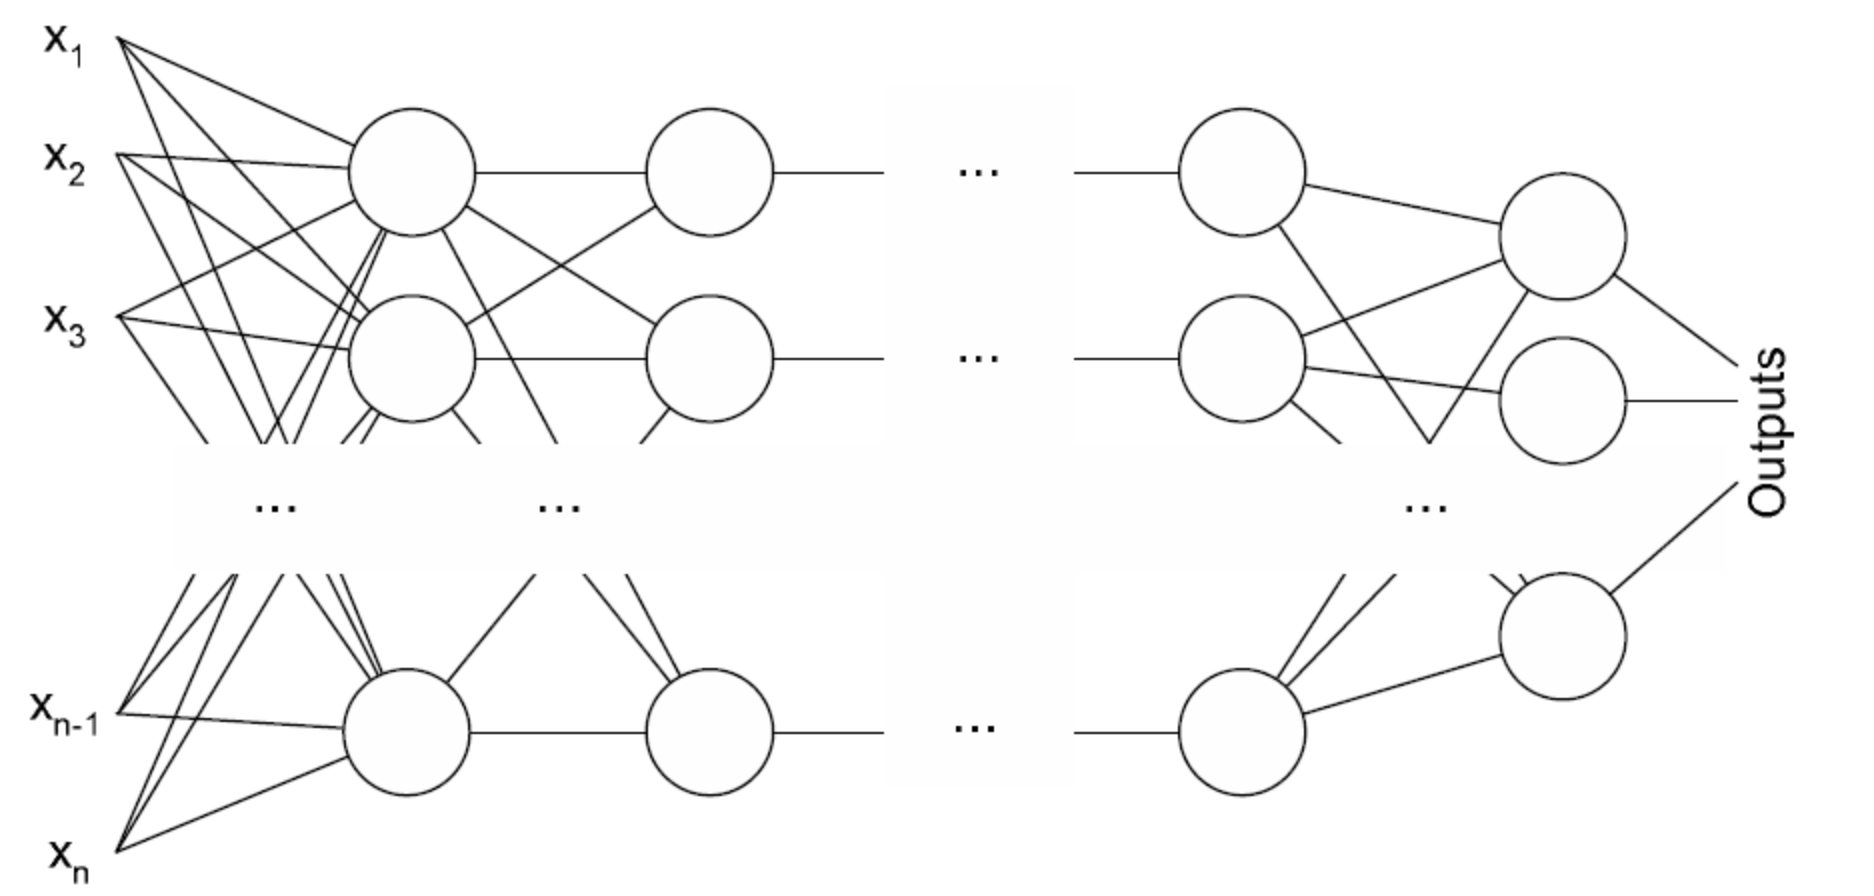
\includegraphics[scale=0.4]{pictures/perseptron.png}
                \caption{Multilayer perceptron}
                \label{fig:my_label}
            \end{figure} 
        \par
        Нейрон принимает каждый такт на свои n входов заряды величиной $x_j = f_j (x)$ . \\ 
        Эти заряды умножаются на веса $w_j$, а затем берется их сумма. У возбуждающего синапса положительный вес, а у тормозящего -- отрицательный. \\
        \begin{figure}[h!]
                \centering
                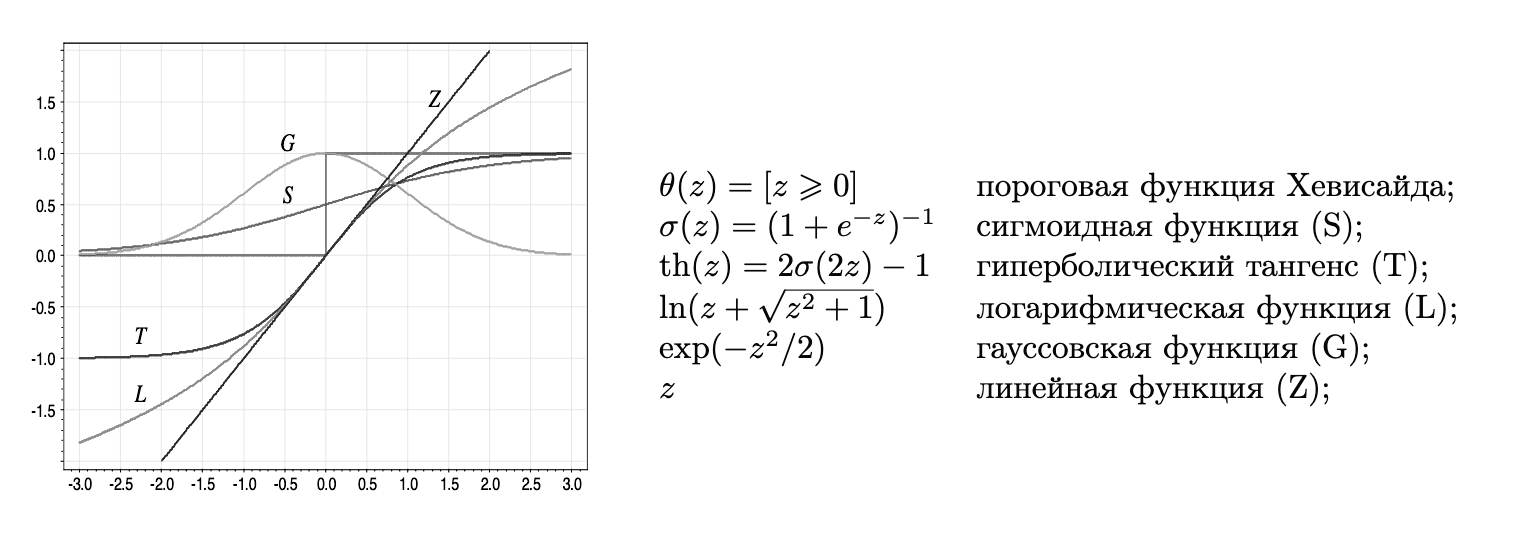
\includegraphics[scale=0.6]{pictures/activation.png}
                \caption{Активационные функции}
                \label{fig:my_label}
            \end{figure} 
        \par
        Если суммарный заряд превышает порог активации $w_0$, то нейрон возбуждается и выдает 1, иначе -1.\\ \\
        \newpage
        \paragraph
        {
        Autoencoder
        }
        \noindent\\
        
        Автоэнкодер -- нейронная сеть, обучающаяся не на отображение в пространство классов, а на самоотображение.\\
        
        \begin{figure}[h!]
                \centering
                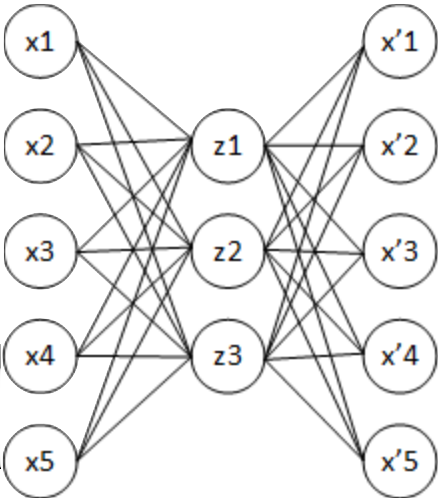
\includegraphics[scale=1]{pictures/autoencoder.png}
                \caption{Примитивный автоэнкодер}
                \label{fig:my_label}
            \end{figure} 
        \par\\
        
        Обучение автоэнкодера происходит путем минимизации ошибки между входным и выходным слоем. \\ \\
        Промежуточные слои автоэнкодера, в отличие от персептрона, должны иметь меньшую размерность, чем входной и выходной слои, для того, чтобы исключенить тривиальность решения.
    \newpage
    \section{Модель данных}
        Данные предоставлены в виде RAW сигналов преамбул с 5-ти различных устройств, расположенных в двух различных местах. \\
        Эти устройства:
        \begin{itemize}
            \item Lenovo
            \item Moto 8
            \item Pixel
            \item Tab 4
            \item Zen
        \end{itemize}\\
        
        Хранятся данные в формате .mat файлов, в структуре данных dict.\\ 
        Обращение к данным производится по полям "$X$" – для получения выборки, и "$y$" – для получения массива классов.
        
        \paragraph{Краткое описание датасета:}
        \begin{itemize}
            \item Приемник – ADALM PLUTO
            \item Передатчики – смартфоны
            \item 5 несбалансированных классов
            \item 2 различных канала
            \item 17281 преамбула
            \item 480 признаков
        \end{itemize}
        \begin{figure}[h!]
                \centering
                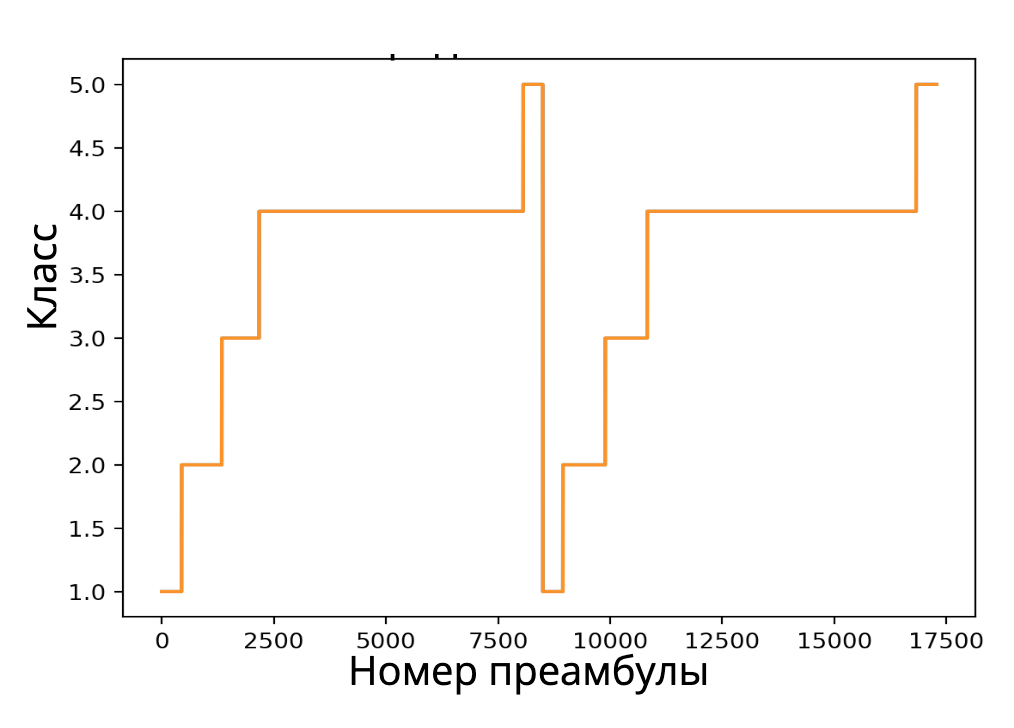
\includegraphics[scale=0.4]{pictures/target.png}
                \caption{График распределения классов}
                \label{fig:my_label}
            \end{figure} 
        \par
